\InputIfFileExists{../data/global.src}\relax\relax

\iffull
\title{TODO}
\subtitle{Tutorium sechs}
\date{KW 24}
\addbibresource{references.bib}
\fi
\SetTutoriumNumber{6}

\iffull\begin{document}
\titleframe

\TopicOverview{7}
\fi

\iffull{\SummaryFrame
\def\sub#1#2{\node[font=\footnotesize\sffamily,scale=.715,align=center,gray,below=-2.65mm] at(#1.south) {\strut#2\strut};}
\setbeamerfont{description item}{series=\mdseries,shape=\itshape}
\begin{frame}[c]{Algorithmen}
\begin{itemize}[<+(1)->]
   \itemsep14pt
   \item Totale Korrektheit \begin{description}[Partielle Korrektheit: ]
      \item[Terminiertheit:] \strut\onslide<+(1)->{Endliche Schritte für jede Eingabe}
      \item[Partielle Korrektheit:] \strut\onslide<+(1)->{Wenn terminiert, dann korrekt}
   \end{description}
   \item Weitere Eigenschaften \begin{description}[Determiniertheit: ]
      \item[Determiniertheit:] \strut\onslide<+(1)->{Gleiche Eingabe~\(\to\) Gleiche Ausgabe}
      \item[Determinismus:] \strut\onslide<+(1)->{Gleiche Eingabe~\(\to\) Gleiche Zustandsfolge}
   \end{description}
\end{itemize}\vfill
\centerline{%
\begin{tikzpicture}
    \onslide<+(1)->{\node (0) at(0,0) {\strut Spezifikation};
    \sub0{Begriffe mit\\Problemrelevanz}}
    \foreach[count=\i,remember =\i as \li (initially 0)] \a/\t in {Abstraktion/{Gegeben \& Gesucht},{\makebox[14mm]{\only<17->{\sbseries}Entwurf}}/{Algorithmus},Verifikation/{Termination \&\\partielle Korrektheit},Aufwandsanalyse/{Laufzeitverhalten}} {
        \onslide<+(1)->{\node[right=.5mm] (k\i) at(\li.east) {\strut\faAngleRight};
        \node[right=.5mm] (\i) at (k\i.east) {\strut\a};
        \sub\i{\t}}
    }
\end{tikzpicture}}
\end{frame}

\def\mto{\ensuremath{\to}}
\def\dt#1{{\textcolor{paletteA!58!white}{\sbseries\strut#1}}}
\begin{frame}[c]{Konstrukte}
\begin{itemize}[<+(1)->]
   \itemsep18pt
   \item \textit{Implizit}:\quad\pause \dt{byte}~\mto~\dt{short}~\mto~\dt{int}~\mto~\dt{long}~\mto~\dt{float}~\mto~\dt{double}\\
   Zahlen von klein zu groß, sowie: \dt{char}~\mto~\dt{int}
   \item \textit{Präzedenzregeln}:\pause\\
   Post vor Prä, sonst wie Arithmetik \& Logik
   \item \textit{Default-Werte}:\quad\pause Zahlen und Zeichen \bjava{0}, Boolean \bjava{false}, Rest \bjava{null}\pause\\
   Nur bei: Arrays, Instanz- und Klassenvariablen (\link{https://docs.oracle.com/javase/specs/jls/se17/html/jls-4.html\#jls-4.12.5}{JLS17~4.12.5})
   \item \textit{Überschatten}:\pause\\
   Lokaler Bezeichner überdeckt Gültigkeit des globalen
\end{itemize}
\end{frame}

\def\mto{\ensuremath{\to}}
\begin{frame}[c]{Arrays \& Iteration}
\begin{itemize}[<+(1)->]
   \itemsep18pt
   \item Arrays sind komplexe Datentypen
   \item Mehrdimensionale Arrays sind eindimensionale Arrays von eindimensionalen Arrays von\ldots
   \item Die drei Schleifenarten sind gleich mächtig \begin{itemize}
      \item Maximum bekannt: \bjava{for}
      \item Mindestens ein mal: \bjava{do}-\bjava{while}
      \item Sonst: \bjava{while}
   \end{itemize}
\end{itemize}
\end{frame}

\begin{frame}[c]{Unterprogramme}
\begin{itemize}[<+(1)->]
   \itemsep18pt
   \item \textit{Überladung:}\quad\pause Gleicher Name, andere Signatur \begin{itemize}
      \item \textit{Signatur:} \pause Name \& Parametertypliste
      \item Müssen zudem in selber Klasse sein (später: Vererbung)
   \end{itemize}
   \item Beim Aufruf macht Java call-by-value: \begin{itemize}
      \item Alle Parameter werden kopiert (Stack)
   \end{itemize}
   \item \bjava{void} gibt als Keyword an, dass die Methode keinen Rückgabetyp hat
\end{itemize}
\end{frame}

\begin{frame}[c]{Objektorientierte Progammierung}
\begin{itemize}[<+(1)->]
   \itemsep18pt
   \item Eine Klasse definiert die Blaupause für Objekte \begin{itemize}
      \item Attribute definieren den Zustand
      \item Methoden definieren den Verhalten
   \end{itemize}
   \item Der Konstruktor baut den initialen Zustand \begin{itemize}
      \item \textit{Instanziierung}: \pause Erzeugen eines neuen Objektes
      \item Wenn keiner: \pause erzeugt Java den leeren Standardkonstruktor
      \item \bjava{this} erlaubt Aufruf von überladenen Konstruktoren
   \end{itemize}
   \item Klassen, Methoden,~\ldots:\quad \textit{Sichtbarkeit} (\bjava{public},~\ldots)
   \item \textit{Gültigkeit}sbereich:\quad Wo die Variablen \say{deklariert sind} (Überschatten,~\ldots)
\end{itemize}
\end{frame}
}\fi

% TODO: make sectionlink auto triggerat start of section
\SetNextSectionText[.75\linewidth]{Ich glaub es bedarf weiterer Animationen.\smallskip\\ --- Break-Down-Flo}
\section{Präsenzaufgabe}
{\taskenum
\begin{frame}[fragile,c]{Präsenzaufgabe}
\begin{aufgabe}{Meine Kleine, du hast Palindrom!}
    \onslide<2->{In dieser Aufgabe sollen Sie eine rekursive Methode implementieren, die überprüfen soll, ob es sich bei dem als Parameter übergebenen String um ein Palindrom handelt. Ein Palindrom ist ein Wort, das vorwärts und rückwärts gelesen identisch ist.} \onslide<3->{Die Überprüfung soll nicht case-sensitive sein, d.h. das Wort \say{Kajak} soll zum Beispiel ein gültiges Palindrom sein.}

    \onslide<4->{Beantworten Sie zudem folgende Fragen bezüglich Ihrer Implementierung:}
    \begin{enumerate}
        \item<5-> Ist Ihre Implementierung ein linear-rekursiver Algorithmus? Warum?
        \item<6-> Ist Ihre Implementierung ein end- oder kopf-rekursiver Algorithmus? Warum?
    \end{enumerate}
\end{aufgabe}
\end{frame}
}

\begin{frame}[c,fragile]{Eine erste Idee}
    \onslide<2->{\only<3->{\color{gray}}In dieser Aufgabe sollen Sie eine {\color{black}rekursive Methode} implementieren, die überprüfen soll, ob es sich bei dem als {\color{black}Parameter übergebenen String} um ein {\color{black}Palindrom} handelt. Ein Palindrom ist ein Wort, das vorwärts und rückwärts gelesen identisch ist. Die Überprüfung soll {\color{black}nicht case-sensitive} sein, d.h. das Wort \say{Kajak} soll zum Beispiel ein gültiges Palindrom sein.}\bigskip

    \onslide<4->{\color{black}Idee:}
    \footnotesize\begin{itemize}
        \item<5-> Prüfe für \(i = 0\) bis \(i = \floor{\sfrac{\text{\bjava{s.length}}}{2}}\), ob \say{\bjava{s[i] == s[s.length - i - 1]}}.
        \item<6-> \bjava{String::toLowerCase()} entweder für jeden Vergleich oder einmal per Hilfsmethode.
        \item<7-> Noch einfacher: Anstelle \bjava{i} zu inkrementieren, löschen wir das erste und letzte Zeichen nach dem Vergleich (via \bjava{String::substring(int, int)}---das Ende ist exklusiv)!
    \end{itemize}
\end{frame}

\begin{frame}[fragile]{Von Palindromen}
\SetupLstHl\lstfs{10}%
\begin{plainjava}
!*\CodeFileMarkerAttach<2->{Palindrome.java}*!
!*\onslide<3->*!public static boolean isPalindrome(String s) { !*\Snode{@helper}*!
!*\onslide<4->*!    return isPalindromeRecursive(s.toLowerCase());
!*\onslide<3->*!}


!*\onslide<6->*!private static boolean isPalindromeRecursive(String s) {
!*\onslide<7->*!    if(s.length() < 2) !*\Snode{@1}*!
!*\onslide<8->*!        return true;
!*\onslide<10->*!    else if(s.charAt(0) != s.charAt(s.length() - 1)) !*\Snode{@2}*!
!*\onslide<10->*!        return false;
!*\onslide<7->*!    else !*\Snode{@3}*!
!*\onslide<9->*!        return isPalindromeRecursive(s.substring(1, s.length() - 1));
!*\onslide<6->*!}!*\onslide<1->*!
\end{plainjava}
\begin{tikzpicture}[@O]
    \onslide<5->{\node[T,yshift=.33mm,right] at(@helper) {die \say{Hilfsmethode}};}

    \onslide<7->{\node[T,yshift=.33mm,right] at(@1) {Basisfall: weniger als zwei Zeichen};}
    \onslide<9->{\node[T,yshift=.33mm,right] at(@2) {Basisfall: kein Palindrom!};}
    \onslide<7->{\node[T,yshift=.33mm,right] at(@3) {Rekursionsfall};}
\end{tikzpicture}
\end{frame}

\iffull
\MakeThePinguExplainIt[text width=7cm]{cap=!hide,glasses=!hide,sunglasses round,eyes shiny,cup=!hide,santa beard,halo,right item angle=-142,staff right length=17mm}{Mit \bjava{:lan:ret:c:urn:ran:} haben wir hier die zurückzugebenden anonymen Variablen referenziert. Generell ist hier das \say{Speichern} der Position für den Aufstieg der Rekursion informal dargestellt.}
\begin{frame}[c,fragile]{Sie Simulantario Sie!}
\sollockinline\SetupLstHl\lstfs{9}\begin{plainjava}
!*\onslide<2->*!!*\MD4*!private static boolean isPalindrome(String s) { !*\rBS<handout:2-4|4->{s=\dq RegalelaGEr\dq }*!
!*\onslide<2->*!    !*\MD5*!return isPalindrom!*\mb{7,38}\mbg[2-3]{8-42}*!eRecursive(s!*\mb6*!.toLowerCase());!*\ml[4]{43}*! !*\rBS<handout:2-3|6-41>{\dq regalelager\dq }~~\rBS<handout:4|43>{true}*!
!*\onslide<2->*!}
!*\onslide<2->*!!*\MD{8,15,20,25,30,35}*!private static boolean isPalindromeRecursive(String s) { !*\rBS<handout:0|8-14>{s=\dq regalelager\dq }\rBS<handout:0|15-19>{s=\dq egalelage\dq }\rBS<handout:0|20-24>{s=\dq galelag\dq }\rBS<handout:2|25-29>{s=\dq alela\dq }\rBS<handout:0|30-34>{s=\dq lel\dq }\rBS<handout:3|35-37>{s=\dq e\dq }*!
!*\onslide<2->*!    !*\MD{9,16,21,26,31,36}*!if(s.length() < 2) return true;!*\ml[3]{37}*!
!*\onslide<2->*!    !*\MD[2]{10,17,22,27,32}*!else if(s.charAt(0) != s.charAt(s.length() - 1)) return false; !*\rBS<handout:0|10-14>{'r'!='r'}\rBS<handout:0|17-19>{'e'!='e'}\rBS<handout:0|22-24>{'g'!='g'}\rBS<handout:2|27-29>{'a'!='a'}\rBS<handout:0|32-34>{'l'!='l'}*!
!*\onslide<2->*!    !*\MD{11,18,23,28,33}*!else return isPalindrom!*\mb{14,19,24,29,34}\mbg[2-3]{15-18,20-23,25-28,30-33,35-41}*!eRecursive(s!*\mb{13}*!.substring(1, s!*\mb{12}*!.length() - 1));!*\ml{38,39,40,41,42}*!
!*\onslide<2->*!}
\end{plainjava}
\only<handout:1|3>{\begin{center}
    \huge\bfseries \say{RegalelaGEr}\\[-2mm]
    {\normalfont\info{Wer sieht auch ein \T{e}, dass die Arme hochwirft?}}
\end{center}}
\begin{onlyenv}<handout:2-4|4-43>\begin{center}\lstfs{6}\lstset{aboveskip=0pt,belowskip=0pt,add to literate={:ll:}{{{\color{lightgray!60!gray}$\ldots$}}}1}
    \begin{tikzpicture}[b/.style={draw=gray,fill=white,text width=4.1cm,minimum height=2.25cm,thick,rounded corners=2pt,inner xsep=1em}]
            \node[b] (a) at(0,0) {%
\begin{plainjava}
!*\MD4*!boolean isPalindrome(String s) {
    !*\MD5*!return isPalindrom!*\mb[1-]{7-42}*!eRecurs!*\mb{6}*!:ll:!*\ml{43-}*!
}
\end{plainjava}\medskip
\centerline{\bjava{s = "RegalelaGEr"}\onslide<43->{ \bjava{:lan:ret:c:urn:ran: = true}}}
            };
\node[above right,gray] at(a.south west) {\(1\)};
\begin{onlyenv}<handout:-3|8-42>\node[b,right=-4cm,yshift=-.1cm] (b) at(a.east) {%
\begin{plainjava}
!*\MD8*!boolean isPalindromeRecursive:ll:
    !*\MD9*!if(s.length() < 2) return:ll:
    !*\MD{10}*!else if(s.charAt(0) != s.c:ll:
    !*\MD{11}*!else return isPalindrom!*\mb[1-]{14-41}*!eRe!*\mb{12-13}*!:ll:!*\ml{42-}*!
}
\end{plainjava}\medskip
\centerline{\bjava{s = "regalelager"}\onslide<42->{ \bjava{:lan:ret:c:urn:ran: = true}}}
        };
\node[above right,gray] at(b.south west) {\(2\)};
    \end{onlyenv}
\begin{onlyenv}<handout:-3|15-41>\node[b,right=-4cm,yshift=-.1cm] (c) at(b.east) {%
\begin{plainjava}
!*\MD{15}*!boolean isPalindromeRecursive:ll:
    !*\MD{16}*!if(s.length() < 2) return:ll:
    !*\MD{17}*!else if(s.charAt(0) != s.c:ll:
    !*\MD{18}*!else return isPalindrom!*\mb[1-]{19-40}*!eRe:ll:!*\ml{41-}*!
}
\end{plainjava}\medskip
\centerline{\bjava{s = "egalelage"}\onslide<41->{ \bjava{:lan:ret:c:urn:ran: = true}}}
        };
\node[above right,gray] at(c.south west) {\(3\)};
    \end{onlyenv}
\begin{onlyenv}<handout:-3|20-40>\node[b,right=-4cm,yshift=-.1cm] (d) at(c.east) {%
\begin{plainjava}
!*\MD{20}*!boolean isPalindromeRecursive:ll:
    !*\MD{21}*!if(s.length() < 2) return:ll:
    !*\MD{22}*!else if(s.charAt(0) != s.c:ll:
    !*\MD{23}*!else return isPalindrom!*\mb[1-]{24-39}*!eRe:ll:!*\ml{40-}*!
}
\end{plainjava}\medskip
\centerline{\bjava{s = "galelag"}\onslide<40->{ \bjava{:lan:ret:c:urn:ran: = true}}}
        };
    \node[above right,gray] at(d.south west) {\(4\)};
    \end{onlyenv}
\begin{onlyenv}<handout:-3|25-39>\node[b,right=-4cm,yshift=-.1cm] (e) at(d.east) {%
\begin{plainjava}
!*\MD{25}*!boolean isPalindromeRecursive:ll:
    !*\MD{26}*!if(s.length() < 2) return:ll:
    !*\MD{27}*!else if(s.charAt(0) != s.c:ll:
    !*\MD{28}*!else return isPalindrom!*\mb[1-]{29-38}*!eRe:ll:!*\ml{39-}*!
}
\end{plainjava}\medskip
\centerline{\bjava{s = "alela"}\onslide<39->{ \bjava{:lan:ret:c:urn:ran: = true}}}
        };
\node[above right,gray] at(e.south west) {\(5\)};
    \end{onlyenv}
\begin{onlyenv}<handout:3|30-38>\node[b,right=-4cm,yshift=-.1cm] (f) at(e.east) {%
\begin{plainjava}
!*\MD{30}*!boolean isPalindromeRecursive:ll:
    !*\MD{31}*!if(s.length() < 2) return:ll:
    !*\MD{32}*!else if(s.charAt(0) != s.c:ll:
    !*\MD{33}*!else return isPalindrom!*\mb[1-]{34-37}*!eRe:ll:!*\ml{38-}*!
}
\end{plainjava}\medskip
\centerline{\bjava{s = "lel"}\onslide<38->{ \bjava{:lan:ret:c:urn:ran: = true}}}
        };
\node[above right,gray] at(f.south west) {\(6\)};
    \end{onlyenv}
\begin{onlyenv}<handout:3|35-37>\node[b,right=-4cm,yshift=-.1cm] (g) at(f.east) {%
\begin{plainjava}
!*\MD{35}*!boolean isPalindromeRecursive:ll:
    !*\MD{36}*!if(s.length() < 2) return:ll:!*\ml[1-]{37-}*!
    else if(s.charAt(0) != s.c:ll:
    else return isPalindromeRe:ll:
}
\end{plainjava}\medskip
\centerline{\bjava{s = "e"}\onslide<37->{ \bjava{:lan:ret:c:urn:ran: = true}}}
        };
\node[above right,gray] at(g.south west) {\(7\)};
    \end{onlyenv}
    \end{tikzpicture}
\end{center}
\end{onlyenv}
\begin{tikzpicture}[remember picture,overlay]
    \onslide<handout:4-|44->{\node[left=-7mm,scale=.8] at(current page.-20) {\usebox\pinguexplainbox};}
\end{tikzpicture}
\end{frame}
\fi

\iffull
\begin{frame}[c,fragile]{Iterativer Ansatz}
    \begin{itemize}[<+(1)->]
        \item Diese Aufgabe lässt sich auch iterativ prüfen.
        \item Für das Palindrom schauen wir für jedes Zeichen \(i\) der \say{linken Hälfte} ob es mit dem gespiegelten \(\text{\T{length}} - i - 1\) der \say{rechten Hälfte} übereinstimmt:
    \end{itemize}
\begin{plainjava}
!*\onslide<4->*!public static boolean isPalindromeIterative(String s) {
!*\onslide<5->*!    s = s.toLowerCase();
!*\onslide<6->*!    for(int i = 0; i < s.length() / 2; i++) {
!*\onslide<7->*!        if(s.charAt(i) != s.charAt(s.length() - i - 1))
!*\onslide<7->*!            return false;
!*\onslide<6->*!    }
!*\onslide<8->*!    return true;
!*\onslide<4->*!}
\end{plainjava}
\end{frame}

\begin{frame}[c,fragile]{Iterativer Ansatz, II}
    \lstfs{10}\begin{itemize}[<+(1)->]
        \item Dies können wir als \only<-9|handout:0>{???}\only<10->{Tail}-Rekursion umschreiben:
    \end{itemize}
\begin{plainjava}
!*\CodeFileMarkerAttach<3->{PalindromeIterative.java}*!
!*\onslide<3->*!public static boolean isPalindrome(String s) {
!*\onslide<4->*!    return helper(s.toLowerCase(), 0);
!*\onslide<3->*!}
!*\onslide<3->*!
!*\onslide<5->*!private static boolean helper(String s, int i) {
!*\onslide<6->*!    if (i >= s.length() / 2)
!*\onslide<6->*!        return true;
!*\onslide<7->*!    if (s.charAt(i) != s.charAt(s.length() - i - 1))
!*\onslide<7->*!        return false;
!*\onslide<8->*!    return helper(s, i + 1);
!*\onslide<5->*!}
\end{plainjava}
\begin{tikzpicture}[overlay, remember picture]
\begin{uncoverenv}<9->
    \node[above left=.925cm,text width=9.65cm,draw=gray,thick,rounded corners=2pt,scale=.65,yshift=.25cm] at(current page.south east) {%
\begin{plainjava}[aboveskip=0pt, belowskip=0pt]
s = s.toLowerCase();
for(int i = 0; i < s.length() / 2; i++) {
    if(s.charAt(i) != s.charAt(s.length() - i - 1))
        return false;
}
return true;
\end{plainjava}
    };
\end{uncoverenv}
\end{tikzpicture}
\end{frame}
\fi

{\taskenum
\begin{frame}{Ja was isses nun?}
\begin{enumerate}[<+(1)->]
    \itemsep12pt
    \item \task{Ist Ihre Implementierung ein linear-rekursiver Algorithmus? Warum?}\pause
    Unser Verfahren ruft sich \emph{höchstens ein mal selbst auf}, damit ist er linear-rekursiv!
    \item \task{Ist Ihre Implementierung ein end- oder kopf-rekursiver Algorithmus? Warum?}\pause
    Der Algorithmus ist End-Rekursiv, da die letzte im Rekursionsfall ausgeführte Operation die Rekursion selbst ist.
    Damit geschieht im Aufstieg nichts mehr.
\end{enumerate}
\end{frame}
}


% \begin{frame}
%     TODO: rekursions arten undZeichnen: TOODO. schauen für anschnitt rekursion und übernahme oder so
%
%     TODO: fehler in lösung irgendwo..
%     TODO: aussicht
% \end{frame}

\SetNextSectionText{Grundlagen der OOP\\Abgabe: \DTMDate{2022-06-07}}
\section{Übungsblatt 6}
\subsection{Aufgabe 1}
{\taskenum
\begin{frame}[c]{Aufgabe 1: Klassenentwurf in Java}
    \task{\begin{itemize}[<+(1)->]
        \itemsep5pt
        \item Erstellen Sie eine Klasse Kreis. Diese soll folgende Eigenschaften und Methoden implementieren: \begin{itemize}
            \item Privaten Instanzvariablen für den Radius, Flächeninhalt und Umfang.
            \item einen öffentlichen Konstruktor, der den Radius des Kreises als Parameter übernimmt, die restlichen
            Eigenschaften daraus ableitet, und die entsprechenden Variablen initialisiert.
            \item get- und set-Methoden für die Instanzvariablen. Dabei soll es nur für den Radius eine set-Methode
            geben und Flächeninhalt und Umfang sollen daraus abgeleitet werden. Stellen Sie sicher, dass nur gültige
            Werte für den Radius (\(r \geq 0\)) akzeptiert werden.
            \item Eine Instanzmethode um die Eigenschaften des Kreises auf der Kommandozeile auszugeben
            \item Eine Instanzmethode die einen Kreisradius als Parameter übernimmt, den entsprechenden Flächeninhalt
            berechnet, das zugehörige Attribut aktualisiert und dieses zurückgibt.
            \item Eine Instanzmethode die einen Kreisradius als Parameter übernimmt, den entsprechenden Umfang berechnet,
            das zugehörige Attribut aktualisiert und dieses zurückgibt.
        \end{itemize}
        \item Erstellen Sie eine weitere Klasse \T{KreisMain}, die den Programmeinstiegspunkt implementiert.
        Lesen Sie über die Kommandozeilenparameter einen Radius ein und instanziieren Sie innerhalb der \T{main} Methode
        ein Objekt der Klasse \T{Kreis} mit dem eingelesenen Radius. Lassen Sie sich die Eigenschaften dieser Instanz
        anzeigen.
    \end{itemize}}
\end{frame}
}

\begin{frame}[c,fragile]{Eine runde Sache!}
\begin{onlyenv}<1-12|handout:1>
\begin{columns}[c,onlytextwidth]
\column{.25\linewidth}
\footnotesize\onslide<3->{1.~Private Instanzvariablen für Radius, Flächeninhalt und Umfang.}\medskip\par
\onslide<6->{2.~öffentlicher Konstruktor, der den Radius des Kreises als Parameter übernimmt, die restlichen Eigenschaften daraus ableitet, und die entsprechenden Variablen initialisiert.}
\column{.05\linewidth}
\column{.7\linewidth}
\SetupLstHl
\begin{plainjava}
!*\onslide<2->*!public class Kreis {
!*\onslide<4->*!   private !*\onslide<5->*!double !*\onslide<4->*!radius;
!*\onslide<4->*!   private !*\onslide<5->*!double !*\onslide<4->*!flaeche;
!*\onslide<4->*!   private !*\onslide<5->*!double !*\onslide<4->*!umfang;

!*\onslide<7->*!   public Kreis(double radius) {
!*\onslide<8->*!       this.radius = radius;
!*\onslide<9->*!       this.flaeche = !*\onslide<10->*!Math.PI * radius * radius!*\onslide<9->*!;
!*\onslide<9->*!       this.umfang = !*\onslide<11->*!2 * Math.PI * radius!*\onslide<9->*!;
!*\onslide<7->*!   }
!*\onslide<12->*!   |ihl|...|ihl|
!*\onslide<2->*!}!*\onslide<1->*!
\end{plainjava}
\end{columns}
\end{onlyenv}
\begin{onlyenv}<13-26|handout:2-3>
\begin{columns}[c,onlytextwidth]
\column{.25\linewidth}
\footnotesize\onslide<14->{3.~get- und set-Methoden für die Instanzvariablen. Dabei soll es nur für den Radius eine set-Methode geben und Flächeninhalt und Umfang sollen daraus abgeleitet werden. Stellen Sie
sicher, dass nur gültige Werte für den Radius (\(r \geq 0\)) akzeptiert werden.}\medskip\par
\column{.05\linewidth}
\column{.7\linewidth}
\SetupLstHl
\begin{onlyenv}<-17|handout:2>
\begin{plainjava}
!*\onslide<13->*!public class Kreis {
!*\onslide<13->*!   |ihl|private double radius, flaeche, umfang;|ihl|
!*\onslide<13->*!   |ihl|private Kreis(double radius)  { ... }|ihl|

!*\onslide<15->*!   public double getRadius() {
!*\onslide<15->*!       return this.radius;
!*\onslide<15->*!   }
!*\onslide<16->*!   public double getFlaeche() {
!*\onslide<16->*!       return this.flaeche;
!*\onslide<16->*!   }
!*\onslide<17->*!   public double getUmfang() {
!*\onslide<17->*!       return this.umfang;
!*\onslide<17->*!   }
!*\onslide<13->*!}!*\onslide<1->*!
\end{plainjava}
\end{onlyenv}
\begin{onlyenv}<18-|handout:3>
\begin{plainjava}
!*\onslide<18->*!public class Kreis {
!*\onslide<18->*!   |ihl|private double radius, flaeche, umfang;|ihl|
!*\onslide<18->*!   |ihl|...|ihl|
!*\onslide<19->*!   public void setRadius(double r) {
!*\onslide<21->*!       if (r < 0)!*\onslide<22->*! return;
!*\onslide<22->*!       this.radius = r;
!*\onslide<23->*!       this.flaeche = !*\onslide<24->*!Math.PI * radius * radius!*\onslide<23->*!;
!*\onslide<25->*!       this.umfang = !*\onslide<26->*!2 * Math.PI * radius!*\onslide<25->*!;
!*\onslide<19->*!   }
!*\onslide<19->*!   public void setUmfang(double umfang) {
!*\onslide<20->*!       this.umfang = umfang;
!*\onslide<19->*!   }
!*\onslide<19->*!   public void setFlaeche(double flaeche) {
!*\onslide<20->*!       this.flaeche = flaeche;
!*\onslide<19->*!   }
!*\onslide<18->*!}!*\onslide<1->*!
\end{plainjava}
\end{onlyenv}
\end{columns}
\end{onlyenv}
\begin{onlyenv}<27-34|handout:4>
\begin{columns}[c,onlytextwidth]
\column{.25\linewidth}
\footnotesize\onslide<28->{4.~Eine Instanzmethode um die Eigenschaften des Kreises auf der Kommandozeile auszugeben.}\medskip\par
\onslide<31->{5.~Eine Instanzmethode die einen Kreisradius als Parameter übernimmt, den entsprechenden
Flächeninhalt berechnet, das zugehörige Attribut aktualisiert und dieses zurückgibt.}
\column{.05\linewidth}
\column{.7\linewidth}
\SetupLstHl
\begin{plainjava}
!*\onslide<27->*!public class Kreis {
!*\onslide<27->*!   |ihl|private double radius, flaeche, umfang;|ihl|
!*\onslide<27->*!   |ihl|...|ihl|

!*\onslide<29->*!   public void print() {
!*\onslide<30->*!      System.out.println("Radius: " + radius + "cm" +
!*\onslide<30->*!           + "\n Fläche: " + flaeche + "cm^2"
!*\onslide<30->*!           + "\n Umfang: " + umfang + "cm");
!*\onslide<29->*!   }

!*\onslide<32->*!   public double berechneFlaeche(double radius) {
!*\onslide<33->*!       this.flaeche = Math.PI * radius * radius;
!*\onslide<34->*!       return this.flaeche;
!*\onslide<32->*!   }
!*\onslide<27->*!}!*\onslide<1->*!
\end{plainjava}
\end{columns}
\end{onlyenv}
\begin{onlyenv}<35-|handout:5>
\begin{columns}[c,onlytextwidth]
\column{.25\linewidth}
\footnotesize\onslide<36->{6.~Eine Instanzmethode die einen Kreisradius als Parameter übernimmt, den entsprechenden
Umfang berechnet, das zugehörige Attribut aktualisiert und dieses zurückgibt.}
\column{.05\linewidth}
\column{.7\linewidth}
\SetupLstHl
\begin{plainjava}
!*\onslide<35->*!public class Kreis {
!*\onslide<35->*!   |ihl|private double radius, flaeche, umfang;|ihl|
!*\onslide<35->*!   |ihl|...|ihl|

!*\onslide<37->*!   public double berechneUmfang(double radius) {
!*\onslide<38->*!       this.umfang = 2 * Math.PI * radius;
!*\onslide<39->*!       return this.umfang;
!*\onslide<37->*!   }
!*\onslide<35->*!}!*\onslide<1->*!
\end{plainjava}
\end{columns}
\end{onlyenv}
\end{frame}

\begin{frame}[c,fragile]{Eine runde Sache?}
\lstfs{7}% adaptive cols
\begin{tikzpicture}[@O]
    % TODO: animations
    \def\hlcolor{pingu@red}
    \onslide<3-8|handout:1-2>{\hlbehindcodeunder{f1}{@f1>}
    \hlbehindcodeunder{f2}{@f2>}
    \hlbehindcodeunder{f3}{@f3>}}
    \def\hlcolor{pingu@blue}
    \onslide<4-8|handout:1-2>{\hlbehindcodeunder{u1}{@f1>}
    \hlbehindcodeunder{u2}{@f2>}
    \hlbehindcodeunder{u3}{@f3>}}
    \def\hlcolor{pingu@yellow}
    \def\hlcolor{pingu@green!82!pingu@black}
\end{tikzpicture}\vspace*{-1.85\baselineskip}
\begin{onlyenv}<2-6|handout:1>
\columns[c,onlytextwidth]
\column{.48\linewidth}
\begin{plainjava}[basicstyle={\solGetStyle{basicstyle}\HStrut}]
public class Kreis {
    private double radius;
    private double flaeche;
    private double umfang;
    public Kreis(double radius) {
        this.radius = radius;
        !*\Snode{f1}*!this.flaeche = Math.PI * radius * radius!*\Snode{f1@}*!;
        !*\Snode{u1}*!this.umfang = 2 * Math.PI * radius!*\Snode{u1@}*!;
    }
    public double getRadius() {
        return this.radius;
    }
    public double getFlaeche() {
        return this.flaeche;
    }
    public double getUmfang() {
        return this.umfang;
    }
    public void setRadius(double r) {
        if (r < 0) return;
        this.radius = r;
        !*\Snode{fla3}*!!*\Snode{f2}*!this.flaeche = Math.PI * radius * radius!*\Snode{f2@}*!;
\end{plainjava}
\column{.52\linewidth}
\begin{plainjava}[basicstyle={\solGetStyle{basicstyle}\HStrut}]
        !*\Snode{umf3}*!!*\Snode{u2}*!this.umfang = 2 * Math.PI * radius!*\Snode{u2@}*!;
    }
    !*\Snode{umf1}*!public void setUmfang(double umfang) {
        this.umfang = umfang;
    !*\Snode{umf1@}*!}
    !*\Snode{fla1}*!public void setFlaeche(double flaeche) {
        this.flaeche = flaeche;
    !*\Snode{fla1@}*!}
    public void print() {
        System.out.println("Radius: " + radius + "cm" +
            + "\n Fläche: " + flaeche + "cm^2"
            + "\n Umfang: " + umfang + "cm");
    }
    !*\Snode{fla2}*!public double berechneFlaeche(double radius) {
        !*\Snode{f3}*!this.flaeche = Math.PI * radius * radius!*\Snode{f3@}*!;
        return this.flaeche;
    !*\Snode{fla2@}*!}
    !*\Snode{umf2}*!public double berechneUmfang(double radius) {
        !*\Snode{u3}*!this.umfang = 2 * Math.PI * radius!*\Snode{u3@}*!;
        return this.umfang;
    !*\Snode{umf2@}*!}
}
\end{plainjava}
\endcolumns
\end{onlyenv}
\begin{onlyenv}<7-8|handout:2>
\columns[c,onlytextwidth]
\column{.48\linewidth}
\begin{plainjava}[basicstyle={\solGetStyle{basicstyle}\HStrut}]
public class Kreis {
    private double radius;
    private double flaeche;
    private double umfang;
    public Kreis(double radius) {
        !*\Snode{r1}*!this.radius = radius;
        !*\Snode{f1}*!berechneFlaeche(radius)!*\Snode{f1@}*!;
        !*\Snode{r1@}*!!*\Snode{u1}*!berechneUmfang(radius)!*\Snode{u1@}*!;
    }
    public double getRadius() {
        return this.radius;
    }
    public double getFlaeche() {
        return this.flaeche;
    }
    public double getUmfang() {
        return this.umfang;
    }
    !*\Snode{r2}*!public void setRadius(double r) {
        if (r < 0) return;
        this.radius = r;
    !*\Snode{r2@}*!    !*\Snode{fla3}*!!*\Snode{f2}*!berechneFlaeche(r)!*\Snode{f2@}*!;
\end{plainjava}
\column{.52\linewidth}
\begin{plainjava}[basicstyle={\solGetStyle{basicstyle}\HStrut}]
    !*\Snode{r3}*!    !*\Snode{umf3}*!!*\Snode{u2}*!berechneUmfang(r)!*\Snode{u2@}*!;
    !*\Snode{r3@}*!}
    !*\Snode{umf1}*!public void setUmfang(double umfang) {
        this.umfang = umfang;
    !*\Snode{umf1@}*!}
    !*\Snode{fla1}*!public void setFlaeche(double flaeche) {
        this.flaeche = flaeche;
    !*\Snode{fla1@}*!}
    public void print() {
        System.out.println("Radius: " + radius + "cm" +
            + "\n Fläche: " + flaeche + "cm^2"
            + "\n Umfang: " + umfang + "cm");
    }
    !*\Snode{fla2}*!public double berechneFlaeche(double radius) {
        !*\Snode{f3}*!this.flaeche = Math.PI * radius * radius!*\Snode{f3@}*!;
        return this.flaeche;
    !*\Snode{fla2@}*!}
    !*\Snode{umf2}*!public double berechneUmfang(double radius) {
        !*\Snode{u3}*!this.umfang = 2 * Math.PI * radius!*\Snode{u3@}*!;
        return this.umfang;
    !*\Snode{umf2@}*!}
}
\end{plainjava}
\endcolumns
\end{onlyenv}
\begin{onlyenv}<9|handout:0>
\columns[c,onlytextwidth]
\column{.48\linewidth}
\begin{plainjava}[basicstyle={\solGetStyle{basicstyle}\HStrut}]
public class Kreis {
    private double radius;
    private double flaeche;
    private double umfang;
    public Kreis(double radius) {
        !*\Snode{r1}*!this.radius = radius;
        berechneFlaeche(radius);
        !*\Snode{r1@}*!berechneUmfang(radius);
    }
    public double getRadius() {
        return this.radius;
    }
    public double getFlaeche() {
        return this.flaeche;
    }
    public double getUmfang() {
        return this.umfang;
    }
    !*\Snode{r2}*!public void setRadius(double r) {
        if (r < 0) return;
        this.radius = r;
    !*\Snode{r2@}*!    berechneFlaeche(r):
\end{plainjava}
\column{.52\linewidth}
\begin{plainjava}[basicstyle={\solGetStyle{basicstyle}\HStrut}]
    !*\Snode{r3}*!    berechneUmfang(r);
    !*\Snode{r3@}*!}
    public void setUmfang(double umfang) {
        this.umfang = umfang;
    }
    public void setFlaeche(double flaeche) {
        this.flaeche = flaeche;
    }
    public void print() {
        System.out.println("Radius: " + radius + "cm" +
            + "\n Fläche: " + flaeche + "cm^2"
            + "\n Umfang: " + umfang + "cm");
    }
    public double berechneFlaeche(double radius) {
        this.flaeche = Math.PI * radius * radius;
        return this.flaeche;
    }
    public double berechneUmfang(double radius) {
        this.umfang = 2 * Math.PI * radius;
        return this.umfang;
    }
}
\end{plainjava}
\endcolumns
\end{onlyenv}
\begin{onlyenv}<10-|handout:3>
\columns[c,onlytextwidth]
\column{.48\linewidth}
\begin{plainjava}[basicstyle={\solGetStyle{basicstyle}\HStrut}]
!*\CodeFileMarkerAttach<11->{Kreis.java}*!
public class Kreis {
    private double radius;
    private double flaeche;
    private double umfang;
    public Kreis(double radius) {
        !*\Snode{r1}*!setRadius(radius);
    }
    public double getRadius() {
        return this.radius;
    }
    public double getFlaeche() {
        return this.flaeche;
    }
    public double getUmfang() {
        return this.umfang;
    }
    !*\Snode{r2}*!public void setRadius(double r) {
        if (r < 0) return;
        this.radius = r;
    !*\Snode{r2@}*!    berechneFlaeche(r);
\end{plainjava}
\column{.52\linewidth}
\begin{plainjava}[basicstyle={\solGetStyle{basicstyle}\HStrut}]
    !*\Snode{r3}*!    berechneUmfang(r);
    !*\Snode{r3@}*!}
    public void setUmfang(double umfang) {
        this.umfang = umfang;
    }
    public void setFlaeche(double flaeche) {
        this.flaeche = flaeche;
    }
    public void print() {
        System.out.println("Radius: " + radius + "cm" +
            + "\n Fläche: " + flaeche + "cm^2"
            + "\n Umfang: " + umfang + "cm");
    }
    public double berechneFlaeche(double radius) {
        this.flaeche = Math.PI * radius * radius;
        return this.flaeche;
    }
    public double berechneUmfang(double radius) {
        this.umfang = 2 * Math.PI * radius;
        return this.umfang;
    }
}
\end{plainjava}
\endcolumns
\end{onlyenv}
\begin{tikzpicture}[@O]
    \onslide<5-7|handout:1>{
        \fill[rounded corners=1.6pt,orange,opacity=\hlopa] ([xshift=-1mm,yshift=5pt]umf1) rectangle ([xshift=-1mm-3.2pt,yshift=-5pt]umf1@);
        \fill[rounded corners=1.6pt,orange,opacity=\hlopa] ([xshift=-1mm,yshift=5pt]umf2) rectangle ([xshift=-1mm-3.2pt,yshift=-5pt]umf2@);
        \fill[rounded corners=1.6pt,orange,opacity=\hlopa] ([xshift=-1mm,yshift=5pt]umf3) rectangle ([xshift=-1mm-3.2pt,yshift=-5pt]umf3);
    }
    \onslide<9|handout:2>{
        \fill[rounded corners=1.6pt,gray!80!pingu@black,opacity=\hlopa] ([xshift=-1mm,yshift=5pt]r1) rectangle ([xshift=-1mm-3.2pt,yshift=-5pt]r1@);
        \fill[rounded corners=1.6pt,gray!80!pingu@black,opacity=\hlopa] ([xshift=-1mm,yshift=5pt]r2) rectangle ([xshift=-1mm-3.2pt,yshift=-5pt]r2@);
        \fill[rounded corners=1.6pt,gray!80!pingu@black,opacity=\hlopa] ([xshift=-1mm,yshift=5pt]r3) rectangle ([xshift=-1mm-3.2pt,yshift=-5pt]r3@);
    }
    \onslide<10-|handout:3>{
        \fill[rounded corners=1.6pt,gray!80!pingu@black,opacity=\hlopa] ([xshift=-1mm,yshift=5pt]r1) rectangle ([xshift=-1mm-3.2pt,yshift=-5pt]r1);
        \fill[rounded corners=1.6pt,gray!80!pingu@black,opacity=\hlopa] ([xshift=-1mm,yshift=5pt]r2) rectangle ([xshift=-1mm-3.2pt,yshift=-5pt]r2@);
        \fill[rounded corners=1.6pt,gray!80!pingu@black,opacity=\hlopa] ([xshift=-1mm,yshift=5pt]r3) rectangle ([xshift=-1mm-3.2pt,yshift=-5pt]r3@);
    }
    \onslide<6-7|handout:1>{
        \fill[rounded corners=1.6pt,gray!70!pingu@black,opacity=\hlopa] ([xshift=-1mm,yshift=5pt]fla1) rectangle ([xshift=-1mm-3.2pt,yshift=-5pt]fla1@);
        \fill[rounded corners=1.6pt,gray!70!pingu@black,opacity=\hlopa] ([xshift=-1mm,yshift=5pt]fla2) rectangle ([xshift=-1mm-3.2pt,yshift=-5pt]fla2@);
        \fill[rounded corners=1.6pt,gray!70!pingu@black,opacity=\hlopa] ([xshift=-1mm,yshift=5pt]fla3) rectangle ([xshift=-1mm-3.2pt,yshift=-5pt]fla3);
    }
\end{tikzpicture}
\end{frame}

\iffull
\begin{frame}{Ja dreht es sich nun?}
    \begin{itemize}[<+(1)->]
        \itemsep6pt
        \item So haben wir noch unzählige Unsauberkeiten: \begin{itemize}
            \item Der \bjava{Kreis(dobule)} prüft nun auch, ob der Radius mindestens \(0\) ist \info{ist das gewollt?}
            \item Mit \bjava{setUmfang(double)} und \bjava{setFlaeche(double)} können wir die abgeleiteten Eigenschaften zerstören
            \item Analog mit \bjava{berechneFlaeche(double)} und \bjava{berechneUmfang(double)}
            \item Wir nutzen ein eigenes \bjava{print} und nicht Javas \bjava{toString}-Mechanismus
        \end{itemize}
        \item Hier kam dies aber einfach durch die Aufgabe\ldots
        \item Die lief ja auch recht gut!
    \end{itemize}
\end{frame}
\fi

\begin{frame}[fragile,c]{Oh halt! Die \T{\textbf{KreisMain.java}}!}
\begin{plainjava}
!*\CodeFileMarkerAttach<7->{KreisMain.java}*!
!*\onslide<2->*!public class KreisMain {
!*\onslide<3->*!   public static void main(String[] args) {
!*\onslide<4->*!       double radius = Double.parseDouble(args[0]);
!*\onslide<5->*!       Kreis k = new Kreis(radius);
!*\onslide<6->*!       k.print();
!*\onslide<3->*!   }
!*\onslide<2->*!}
\end{plainjava}
\end{frame}

\subsection{Aufgabe 2}
{\taskenum
\begin{frame}[fragile]{Aufgabe 2: Gültigkeitsbereiche von Variablen}
\begin{enumerate}[<+(1)->]
    \item \task{Betrachten Sie folgende Klassendefinition:}
\begin{plainjava}
!*\onslide<3->*!public class DemoA {
!*\onslide<3->*!    static int x = 0;
!*\onslide<3->*!    int y = 1;
!*\onslide<3->*!    public static int methode(int z){
!*\onslide<3->*!        return this.y + z;
!*\onslide<3->*!    }
!*\onslide<3->*!}
\end{plainjava}
    \task<4->{Handelt es sich hierbei um eine gültige Java Klassendefinition? Begründen Sie Ihre Antwort \textit{kurz}.}
\end{enumerate}
\end{frame}


\begin{frame}[fragile]{Und nun Ausgaben!}
\begin{enumerate}[<+(1)->]
    \setcounter{enumi}{1}
    \item \task{Betrachten Sie folgende Klassendefinition:}
\begin{plainjava}
!*\onslide<3->*!public class DemoB {
!*\onslide<3->*!    int x = 0;
!*\onslide<3->*!    public static void methode(int x){
!*\onslide<3->*!        System.out.println(x);
!*\onslide<3->*!    }
!*\onslide<3->*!    public static void methode2(){
!*\onslide<3->*!        methode(1);
!*\onslide<3->*!    }
!*\onslide<3->*!    public static void main(String[] args){
!*\onslide<3->*!        methode2();
!*\onslide<3->*!    }
!*\onslide<3->*!}
\end{plainjava}
    \task<4->{Welche Ausgabe erzeugt das Programm? Begründen Sie Ihre Antwort \textit{kurz}.}
\end{enumerate}
\end{frame}

\begin{frame}[fragile]{Und nochmal Ausgaben!}
\begin{enumerate}[<+(1)->]
    \setcounter{enumi}{2}
    \item \task{Betrachten Sie folgende Klassendefinition:}
\begin{plainjava}
!*\onslide<3->*!public class DemoC {
!*\onslide<3->*!    static int i;
!*\onslide<3->*!    public static void methode(){
!*\onslide<3->*!        for(; i <= 3; i++){
!*\onslide<3->*!            System.out.println(i);
!*\onslide<3->*!        }
!*\onslide<3->*!    }
!*\onslide<3->*!    public static void main(String[] args){
!*\onslide<3->*!        methode();
!*\onslide<3->*!        methode();
!*\onslide<3->*!    }
!*\onslide<3->*!}
\end{plainjava}
    \task<4->{Welche Ausgabe erzeugt das Programm? Begründen Sie Ihre Antwort \textit{kurz}.}
\end{enumerate}
\end{frame}
}

\iffull
\SetNextSectionText{Grundlagen der Rekursion\\Abgabe: \DTMDate{2022-06-20}}
\section{Aussicht: Übungsblatt 7}
\begin{frame}{Habbeldu}
\end{frame}
\fi

\SetNextSectionText[.55\linewidth]{TODO}
\section{Abschließendes}
{\SummaryFrame
\begin{frame}[t]{Zusammenfassend}
\pause \printBibCommand
\vfill\vfill % double fill for more fraction
\begin{itemize}[<+(1)->]
    \itemsep5pt
    \item TODO
\end{itemize}
\end{frame}
}

% TODO: pascal case


\outro{\vskip9mm\centering \onslide<2->{\scalebox{1.35}{\begin{tikzpicture}
       % TODO
    \end{tikzpicture}}}}

\iffull\end{document}\fi
